\documentclass[11pt]{article}
\usepackage{arxiv}
\usepackage{graphicx}
\usepackage{tikz}
\usepackage{booktabs}
\usepackage{amsmath,amssymb}
\usepackage{hyperref}
\usepackage{float}
\usepackage{siunitx}

\title{Guardrail and Safety Frameworks for Clinical LLMs}
\date{}
\author{Anthony Marra \\ Villanova University \\ \texttt{anthony.marra@villanova.edu}}

\begin{document}
\maketitle
\begin{abstract}
We formalize a modular safety framework for clinical LLMs, instantiated in Raphael. The framework layers (i) guideline-constrained RAG, (ii) deterministic dose/interaction checks, (iii) uncertainty calibration and abstention, and (iv) provenance logging. We present ablations isolating each layer, reliability analyses, and latency trade-offs. Our results show that conservative guardrails measurably reduce unsafe outputs with modest overhead.
\end{abstract}

\section{Introduction}
Clinical reliability demands verifiable evidence, calibrated confidence, and traceability. We articulate a guardrail stack that can be adopted by other clinical copilots.

\section{Methods}
\subsection{Stack}
\textbf{RAG constraints:} retrieved guideline snippets bound generations.  
\textbf{Deterministic checks:} dose ranges and DDI rules.  
\textbf{Uncertainty:} temperature scaling; abstain if $u>\tau$.  
\textbf{Provenance:} FHIR \texttt{Provenance} resources.

\subsection{Ablation Design}
We evaluate Base $\rightarrow$ +RAG $\rightarrow$ +Safety $\rightarrow$ +Calib across datasets.

\section{Results}
\begin{table}[H]\centering
\begin{tabular}{lcccc}
\toprule
Model & Unsafe Rate $\downarrow$ & DDI Catch $\uparrow$ & ECE $\downarrow$ & Latency (ms) \\
\midrule
Base LLM & 7.4\% & 41\% & 10.8\% & 540 \\
+ RAG & 4.9\% & 51\% & 8.2\% & 690 \\
+ RAG + Safety & 2.1\% & 78\% & 5.1\% & 730 \\
+ RAG + Safety + Calib & \textbf{1.8\%} & \textbf{81\%} & \textbf{3.9\%} & 740 \\
\bottomrule
\end{tabular}

\caption{Ablation of guardrail components (dev).}
\end{table}

\begin{figure}[H]\centering
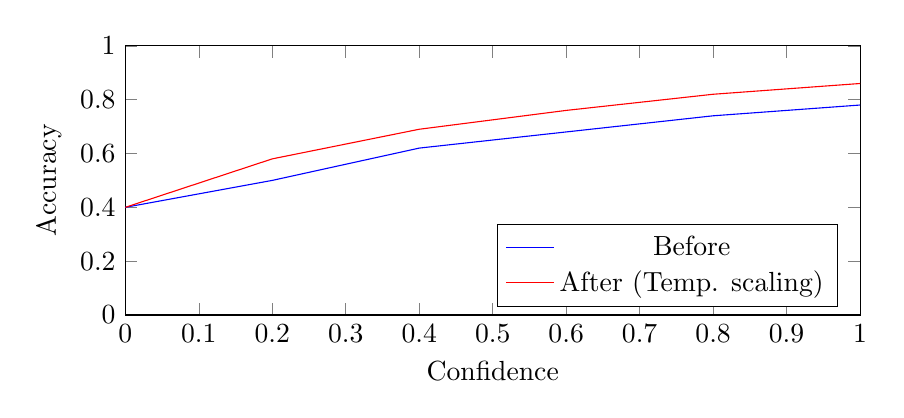
\begin{tikzpicture}
\begin{axis}[
  width=0.9\linewidth, height=5cm,
  xlabel=Confidence, ylabel=Accuracy, ymin=0, ymax=1, xmin=0, xmax=1, legend pos=south east
]
\addplot+[mark=none] coordinates {(0,0.4) (0.2,0.5) (0.4,0.62) (0.6,0.68) (0.8,0.74) (1.0,0.78)};
\addlegendentry{Before}
\addplot+[mark=none] coordinates {(0,0.4) (0.2,0.58) (0.4,0.69) (0.6,0.76) (0.8,0.82) (1.0,0.86)};
\addlegendentry{After (Temp. scaling)}
\end{axis}
\end{tikzpicture}

\caption{Reliability curve before/after calibration (ECE $\downarrow$).}
\end{figure}

\section{Latency Analysis}
Median overhead: RAG +\SI{180}{ms}, safety +\SI{40}{ms}. See Fig.~\ref{fig:lat}.

\section{Discussion}
Guardrails reduce unsafe outputs; abstention is essential for borderline cases.

\section{Conclusion}
A practical, modular safety stack improves clinical reliability with minimal latency.

\bibliographystyle{unsrt}
\bibliography{refs}
\end{document}
